
\subsubsubsection{Applying the Dataflow-oriented Approach with PROV-DfA}

Now we apply the concepts defined in Sections \ref{subsec_datacentric} and \ref{user_steering_def}
to put the PROV-DfA provenance data diagram into practice to illustrate with a concrete example of its use in the libMesh-sedimentation workflow.

In Figure \ref{fig:libmesh_with_provdfa}, we show large raw input files (with mesh data) stored on disk,
with pointers in the solver's input dataset $I_{DS}$.
$I_{DS}$ has over 70 parameters, among which only two are displayed in the figure
(flow linear and non-linear tolerance).
These solver parameters are extracted from a configurations file, which is
read at each iteration.
Yet, the maximum number of iterations ($t_{max}$) is a $L_I$ attribute of the
data transformation solver.
Metadata are extracted ($V_I$) from input raw files at runtime to allow for tracking
their contents while they are processed.
Elements of $O_{DS}$ of each data transformation are also collected
(via raw data extractors and source code instrumentation) and stored in the database.
For example, the solver $O_{DS}$ contains calculated values,
such as linear and non-linear results, as well as the current time iteration value.
In addition to online data analyses, the user performs several adaptations during the simulation.

\begin{figure}[H]
    \centering
    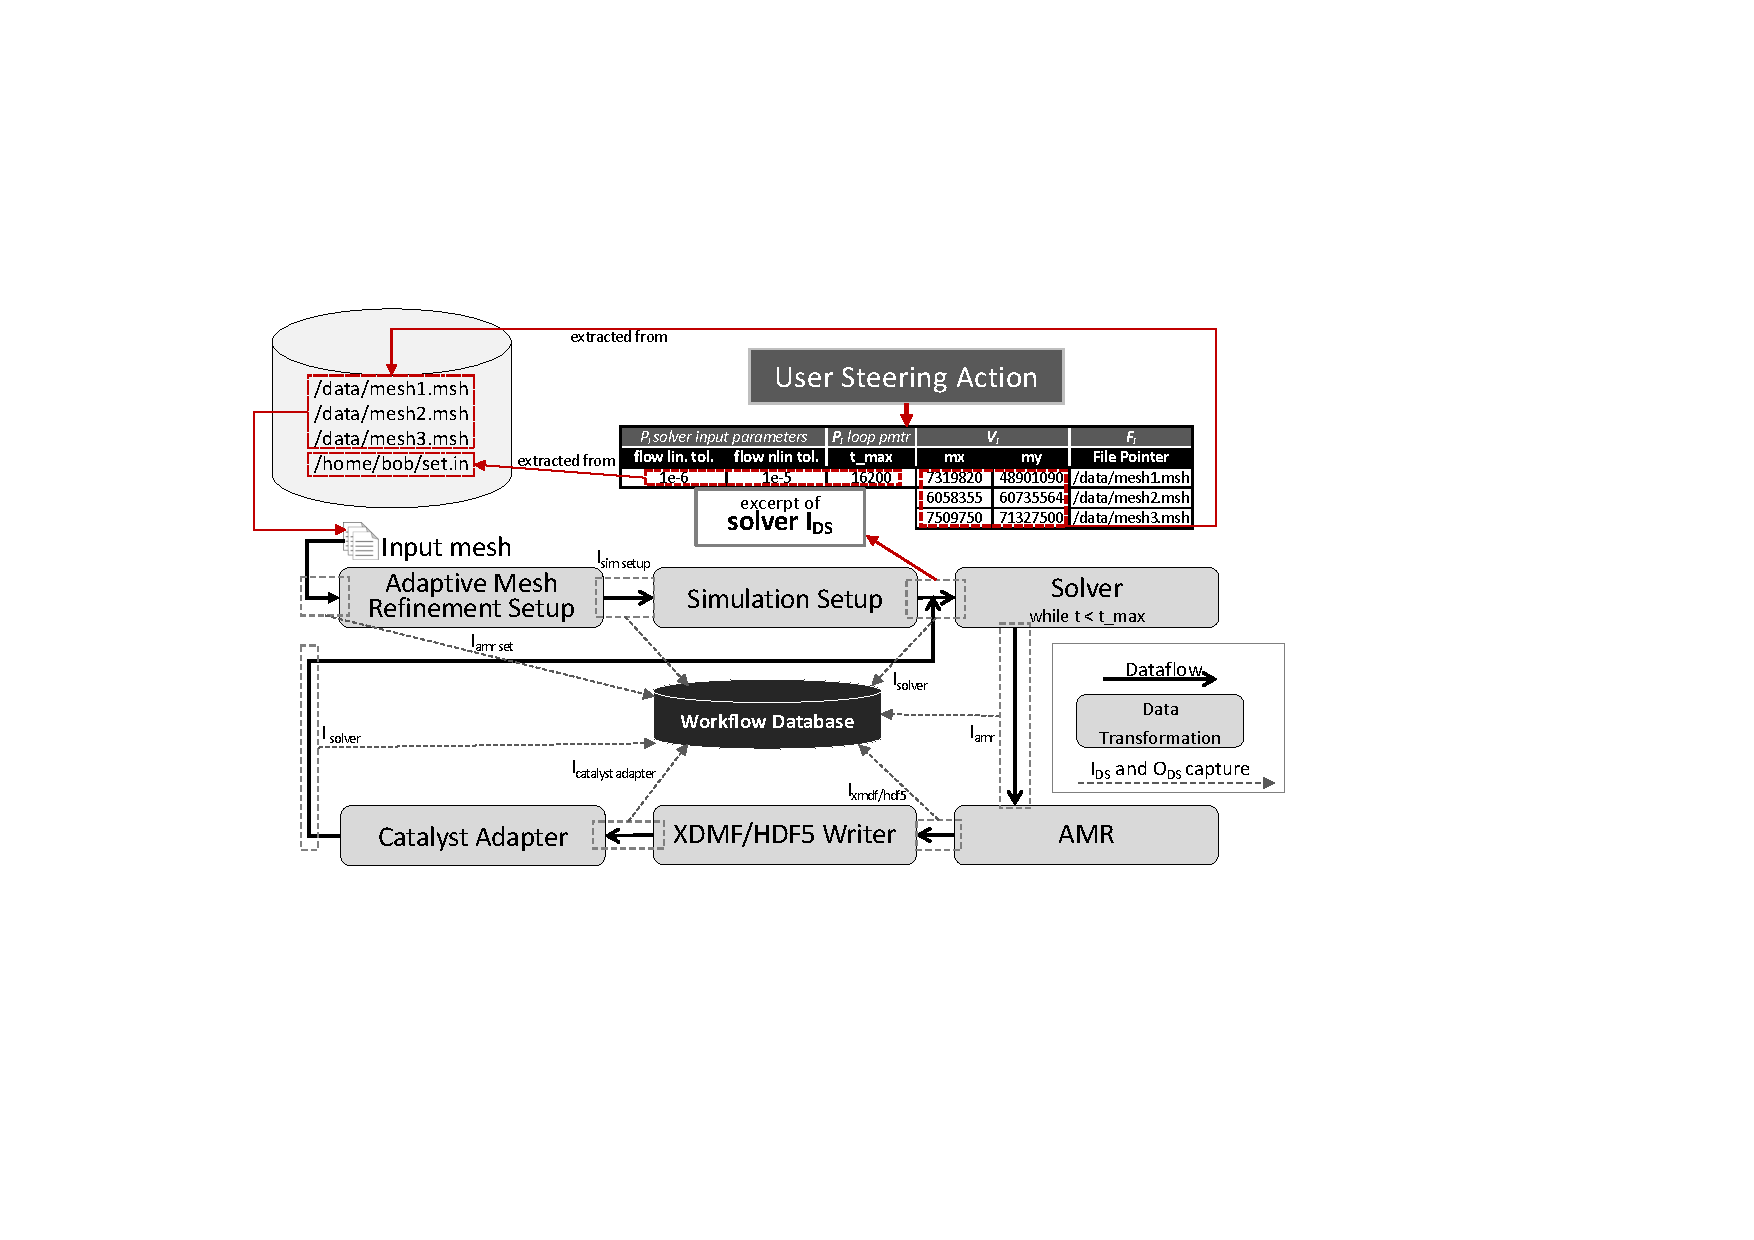
\includegraphics[width=\textwidth,keepaspectratio]{img/steeringaction-provdfa.pdf}
    \caption{Dataflow in the libMesh-sedmentation simulation using the dataflow-oriented approach with PROV-DfA.}
    \label{fig:libmesh_with_provdfa}
\end{figure}

In Figure \ref{fig:visualization_using_provdfa},
we present a visualization of an excerpt of the data in a workflow database
implementing PROV-DfA.
It shows a user tuning the flow linear tolerance parameter from $\num{1e-5}$ to
$\num{1e-3}$ and a data reduction with criteria $mx < \num{7e6}$.


\begin{figure}
    \centering
    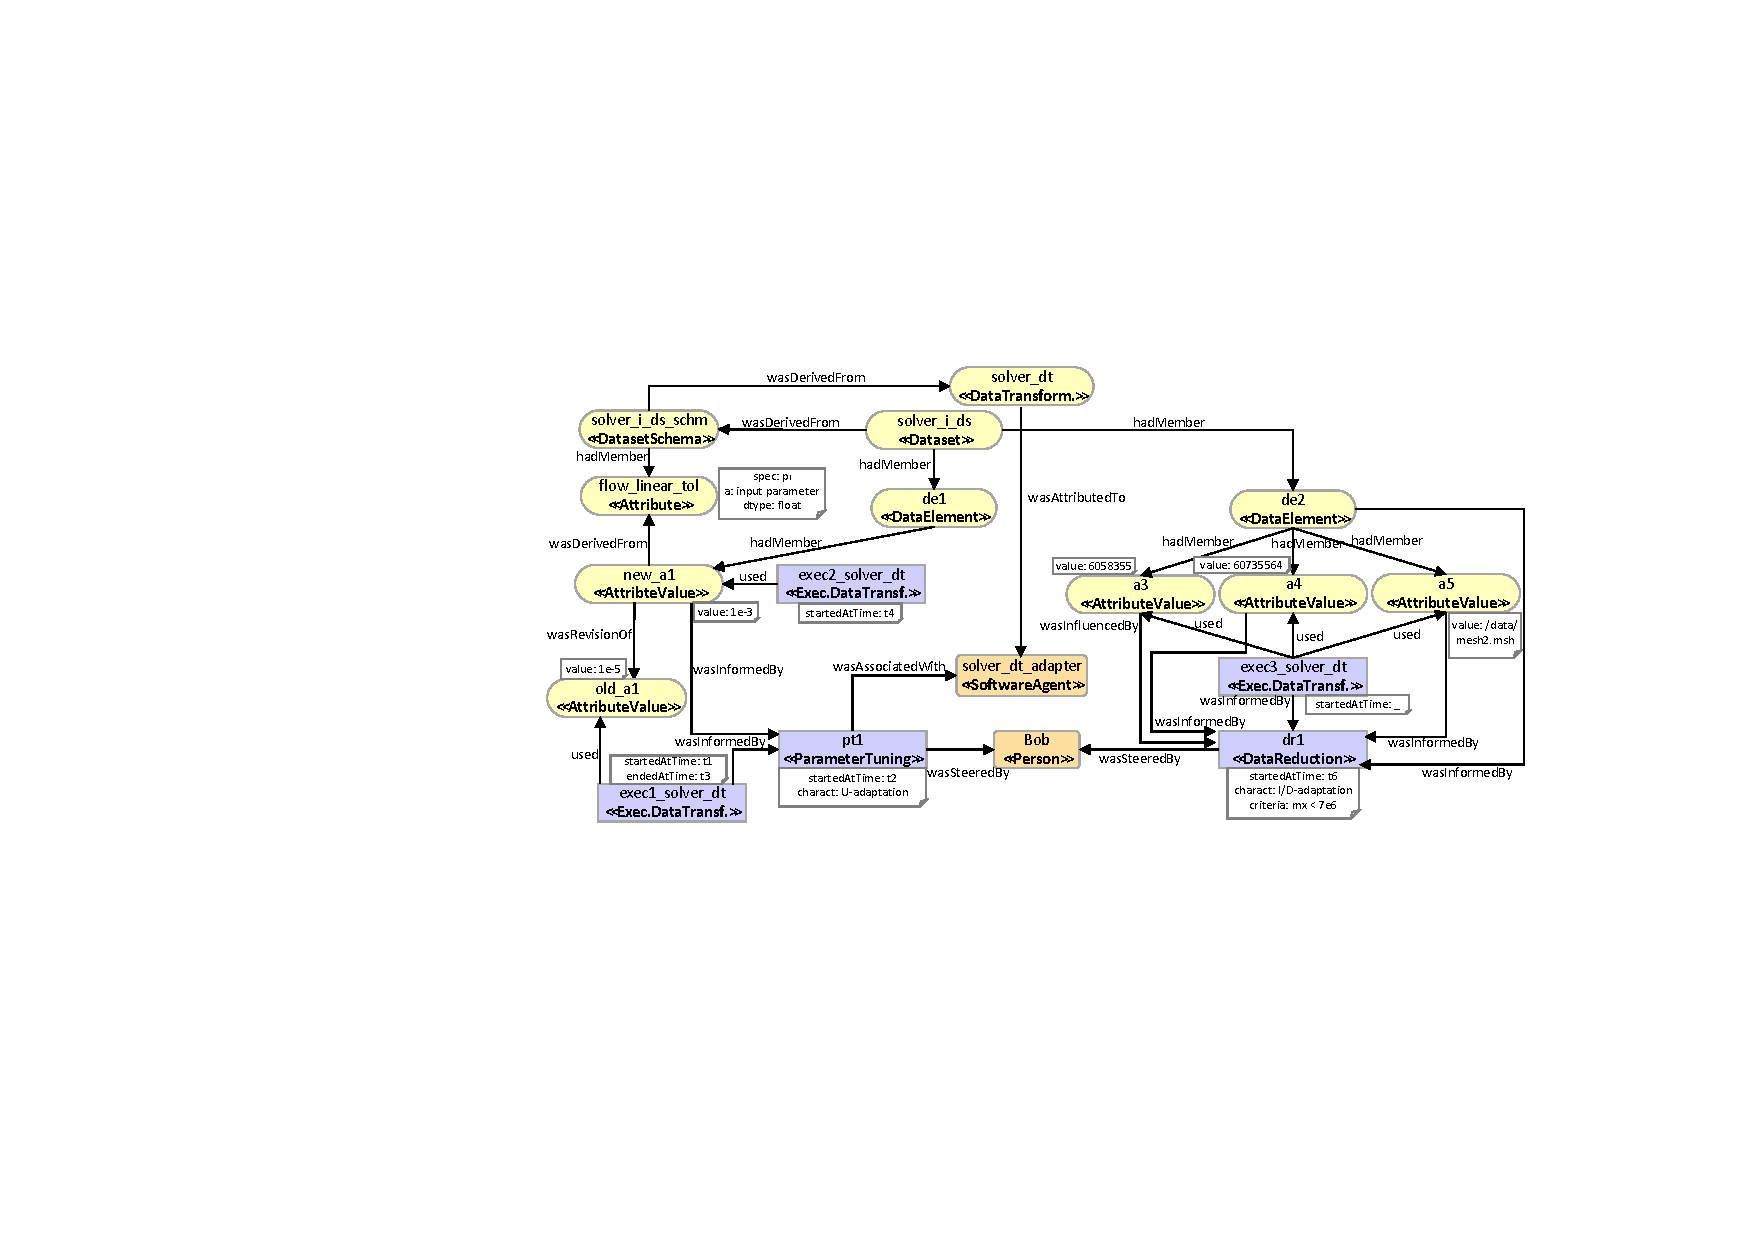
\includegraphics[width=\textwidth,keepaspectratio]{img/PROV-DFA-EXAMPLE.pdf}
    \caption{Visualization of data using PROV-DfA.}
    \label{fig:visualization_using_provdfa}
\end{figure}


By using data in a relational workflow database implementing PROV-DfA,
users can run the following queries (their SQL codes are on GitHub \cite{PROV-DfA_GitHub}).


\begin{itemize}
    \setlength\itemsep{-2mm}
    \item[-] \noindent
    \textit{Inspecting parameter tunings (``who", ``when", ``what")}

    How many tunings did the user do? Which parameters did the user change?
    What were the values when the user changed and what values did the user change into?
    When did each adaptation happen?

    \item[-] \noindent
    \textit{Inspecting parameter tunings (``how")}

    In parameter tuning 3, how was the main solver output values 10 iterations before and after?

    \item[-] \noindent
    \textit{Data reduction (``how", ``which")}

    On average, how long iterations were lasting before and after the user
    reduced input files from the input data? Which files were affected?

\end{itemize}

These queries show the potential of PROV-DfA for workflow databases allowing for tracking user steering action data in large-scale workflows.

